\documentclass{article}
        \usepackage[margin=1in]{geometry}
        \usepackage{algorithm}
        \usepackage{algorithmic}
        \usepackage{hyperref}
        \usepackage{amsmath,amsfonts,amssymb,amsthm,commath,dsfont}
        \usepackage{bm}
        \usepackage{enumitem}
        \usepackage{framed}
        \usepackage{xspace}
        \usepackage{microtype}
        \usepackage{float}
        \usepackage[round]{natbib}
        \usepackage{cleveref}
        \usepackage[dvipsnames]{xcolor}
        \usepackage{graphicx}
        \usepackage{listings}
        \usepackage[breakable]{tcolorbox}
        \tcbset{breakable}
        \usepackage{mathtools}
        \usepackage{autonum}
        \usepackage{comment}
        \usepackage{booktabs}
        \usepackage{enumitem}

        \newlist{legal}{enumerate}{10}
        \setlist[legal]{label*=\arabic*.}
        
        \newcommand{\colbar}{\rule[-3mm]{.3mm}{1.5em}}
        \newcommand{\rowbar}{\rule[.5ex]{1.5em}{.3mm}}
        \newcommand{\francis}[1]{{\color{blue}#1}}
        \DeclareMathOperator{\rank}{rank}
        
        \newcommand{\yb}[1]{{\color{blue} #1}}

        % following loops. stolen from djhsu
        \def\ddefloop#1{\ifx\ddefloop#1\else\ddef{#1}\expandafter\ddefloop\fi}
        % \bbA, \bbB, ...
        \def\ddef#1{\expandafter\def\csname bb#1\endcsname{\ensuremath{\mathbb{#1}}}}
        \ddefloop ABCDEFGHIJKLMNOPQRSTUVWXYZ\ddefloop
        
        % \cA, \cB, ...
        \def\ddef#1{\expandafter\def\csname c#1\endcsname{\ensuremath{\mathcal{#1}}}}
        \ddefloop ABCDEFGHIJKLMNOPQRSTUVWXYZ\ddefloop
        
        % \vA, \vB, ..., \va, \vb, ...
        \def\ddef#1{\expandafter\def\csname v#1\endcsname{\ensuremath{\boldsymbol{#1}}}}
        \ddefloop ABCDEFGHIJKLMNOPQRSTUVWXYZabcdefghijklmnopqrstuvwxyz\ddefloop
        
        % \valpha, \vbeta, ...,  \vGamma, \vDelta, ...,
        \def\ddef#1{\expandafter\def\csname v#1\endcsname{\ensuremath{\boldsymbol{\csname #1\endcsname}}}}
        \ddefloop {alpha}{beta}{gamma}{delta}{epsilon}{varepsilon}{zeta}{eta}{theta}{vartheta}{iota}{kappa}{lambda}{mu}{nu}{xi}{pi}{varpi}{rho}{varrho}{sigma}{varsigma}{tau}{upsilon}{phi}{varphi}{chi}{psi}{omega}{Gamma}{Delta}{Theta}{Lambda}{Xi}{Pi}{Sigma}{varSigma}{Upsilon}{Phi}{Psi}{Omega}{ell}\ddefloop

        \newcommand\T{{\scriptscriptstyle\mathsf{T}}}
        \def\diag{\textup{diag}}
        \newcommand{\bx}{{\boldsymbol x}}
        \newcommand{\xup}[1]{x^{({#1})}}
        \newcommand{\yup}[1]{y^{({#1})}}
        \newcommand{\bxup}[1]{{\bx}^{({#1})}}
        \DeclareMathOperator*{\argmin}{arg\,min}
        \DeclareMathOperator*{\argmax}{arg\,max}

        \def\SPAN{\textup{span}}
        \def\tu{\textup{u}}
        \def\R{\mathbb{R}}
        \def\E{\mathbb{E}}
        \def\Z{\mathbb{Z}}
        \def\be{\bm{e}}
        \def\nf{\nabla f}
        \def\veps{\varepsilon}
        \def\cl{\textup{cl}}
        \def\inte{\textup{int}}
        \def\dom{\textup{dom}}
        \def\Rad{\textup{Rad}}
        \def\lsq{\ell_{\textup{sq}}}
        \def\hcR{\widehat{\cR}}
        \def\hcRl{\hcR_\ell}
        \def\cRl{\cR_\ell}
        \def\hcE{\widehat{\cE}}
        \def\cEl{\cE_\ell}
        \def\hcEl{\hcE_\ell}
        \def\eps{\epsilon}
        \def\1{\mathds{1}}
        \newcommand{\red}[1]{{\color{red} #1}}
        \newcommand{\blue}[1]{{\color{blue} #1}}
        \def\srelu{\sigma_{\textup{r}}}
        \def\vsrelu{\vec{\sigma_{\textup{r}}}}
        \def\vol{\textup{vol}}

        \newcommand{\ip}[2]{\left\langle #1, #2 \right \rangle}
        \newcommand{\mjt}[1]{{\color{blue}\emph\textbf{[M:}~#1~\textbf{]}}}
        \newcommand{\sahand}[1]{{\color{green}\emph\textbf{[Sah:}~#1~\textbf{]}}}

        \newtheorem{fact}{Fact}
        \newtheorem{lemma}{Lemma}
        \newtheorem{claim}{Claim}
        \newtheorem{proposition}{Proposition}
        \newtheorem{theorem}{Theorem}
        \newtheorem{corollary}{Corollary}
        \newtheorem{condition}{Condition}
        \theoremstyle{definition}
        \newtheorem{definition}{Definition}
        \theoremstyle{remark}
        \newtheorem{remark}{Remark}
        \newtheorem{example}{Example}

 

        \newenvironment{Q}
        {%
          \clearpage
          \item
        }
        {%
          \phantom{s} 
          \bigskip
          % \textbf{Solution.}
        }

        \title{CS 446 / ECE 449 --- Homework 1}
        \author{\emph{aidansa2}}
        \date{Version 1.0}

        \begin{document}
        \maketitle

        \noindent\textbf{Instructions.}
        \begin{itemize}
          \item
            Homework is due \textbf{Wednesday, September $17^{th}$, 11:59 a.m}; you have \textbf{3} late days in total for \textbf{all Homeworks}.
        
          \item
            Everyone must submit \textbf{individually} at gradescope under \texttt{hw1}. 

        
          \item
            The ``written'' submission at \texttt{hw1} \textbf{must be typed}, and submitted in
            any format gradescope accepts (to be safe, submit a PDF).  You may use \LaTeX, markdown,
            google docs, MS word, whatever you like; but it must be typed!
        
          \item
            When submitting at \texttt{hw1}, gradescope will ask you to \textbf{mark out boxes
            around each of your answers}; please do this precisely!
        
          \item
            Please make sure your NetID is clear and large on the first page of the homework.
        
          \item
            Your solution \textbf{must} be written in your own words.
            Please see the course webpage for full \textbf{academic integrity} information.
            You should cite any external reference you use.
        

           
        \end{itemize}

        
\begin{enumerate}[font={\Large\bfseries},left=0pt]






\begin{Q}
\textbf{\Large $K$-NN } (43 pt.) 
\begin{enumerate}
    \item Assume that we have a dataset with two labels. The training set comes from the input space which is in the form of Figure~\ref{fig:circle}. Each input sample is within the region enclosed by either of the circles. Each circle represents one class: all the samples that come from the left circle (blue one) are labeled as $0$ and all the samples that come from the right circle (green one) are labeled as $1$. 
    \begin{enumerate}
        \item We know we have $N$ total of training samples, but we do not know how many of them come from each class. We are given a single point from the green circle as well as access to a $K$-NN classifier for which we can choose arbitrary $K$ and query the label of the $K$-NN classifier for the given point. What is the \textbf{minimum} number of queries required (in terms of $N$) to determine the number of training points from each class? 
        Note that at each step, we can choose any $K$ and query the $K$-NN classifier for the label of the test sample, i.e. from the green circle. Explain your answer.  You may assume the number of green points is less than $N/2$. (6 pt.)\\
        \textit{Hint:} Can we do better than $\mathcal{O}(N)$?
        \item  Is there any setting (the number of training samples, their label distribution, etc.) that leads to the wrong prediction for a given test point using $1$-NN classifier?  (4 pt.)
    \end{enumerate}
    

    \begin{figure}[ht!]
        \centering
        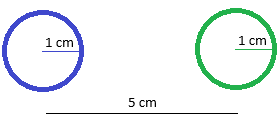
\includegraphics[width=0.5\linewidth]{circles_knn.png}
        \caption{$K$-NN Training Dataset}
        \label{fig:circle}
    \end{figure}

 

    \item 
    Consider a set of data points in $\mathbb{R}^3$ (see Table~\ref{tab:perceptron})\label{}, now we want to use $K$-nearest neighbors ($K$-NN) to classify points in $\mathbb{R}^3$. Answer the questions below.
    \begin{table}[!htb]
            \centering
            \begin{tabular}{|c|c|c|c|c|}
                \hline
                \textbf{Index} & \textbf{$x_1$} & \textbf{$x_2$} & \textbf{$x_3$} & \textbf{Label} \\
                \hline
                1 & 1 & 1 & 1 & 1\\
                \hline
                2 & 0 & 0 & 1 & 1\\
                \hline
                3 & 0 & 0 & 0 & -1\\
                \hline
                4 & 1 & 0 & 0 & -1\\
                \hline
                5 & 0 & 1 & 0 & -1\\
                \hline
            \end{tabular}
            \caption{A set of data points}
            \label{tab:perceptron}
        \end{table}
    \begin{enumerate}
        \item If $K$ = 1, if you have a new data point $\bm{x} = (0.4, 0.4, 1.5)$, what would the label of $\bm{x}$ be? (Please use Euclidean distance as the distance metric for this question.) (3 pt.)

        \item When there is more noise in the training dataset, to reduce the overfitting problem, should we choose smaller $K$ or larger $K$? Please explain your answer. (3 pt.)

    \end{enumerate}
\item
 Assume an input space \(S=\{\bx^{(i)}\}_{i=1}^N\), all $\bx^{(i)}$ being distinct. For each \(\bx^{(i)}\),
the label \(y^{(i)}\in\{1,2\}\) is drawn independently with
\(\mathbb{P}(y^{(i)}=1\,|\,\bx^{(i)})=0.9\).
We form a training set \(\mathcal D=\{(\bx^{(i)},y^{(i)})\}_{i=1}^N\).
Given a test sample \((\bx,y)\) where \(\bx\in S\) and \(y\) is drawn independently with the same conditional distribution, a \(1\)-NN classifier predicts the label $\hat{y}$ of the \(\bx\).
 What would be the probability that we get the correct prediction for $\bx$?
  (8 pt.)\\
 \textit{Hint}: Note that from the assumptions, we know that $\exists (\bx^{(j)}, y^{(j)}) \in \mathcal{D}, \bx^{(j)} = \bx$.



\item
Consider the same setting of (c) but 
now suppose for each \(\bx^{(i)}\in S\) we have \emph{three independent labeled replicas}
\[
(\bx^{(i)},y^{(i,1)}),\;(\bx^{(i)},y^{(i,2)}),\;(\bx^{(i)},y^{(i,3)}),
\]
where each \(y^{(i,r)}\) is drawn independently with
\(\mathbb{P}(y^{(i,r)}=1\,|\,\bx^{(i)})=0.9\).
Let the training set be
\(\mathcal D=\{(\bx^{(i)},y^{(i,r)}):  r=1,2,3\}_{i=1}^{N}\).
Given a test sample \((\bx,y)\) where \(\bx\in S\) and \(y\) is drawn independently with the same conditional distribution,
what would be the probability that a $3$-NN classifier makes the correct prediction for a test sample $\bx$? How does this probability compare to using $1$-NN? (8 pt.)

\textit{Hint}: Note that from the assumptions, we know that $\exists (\bx^{(j)}, y^{(j)}) \in \mathcal{D}, \bx^{(j)} = \bx$.
\item In real-world scenarios, it is common for test data points to have missing features (e.g., due to sensor failure or incomplete measurements). Is it still possible to apply the $K$-NN algorithm in such situations? If so, describe give one of the ways of how this can be achieved. (5 pt.)

\item \textbf{(Bonus question)} Assume an input space $S$ to be a polytope with $N$ vertices in $\R^d$. Further, assume that no pair of vertices are farther apart than $1$ from one another. We are interested in training a $1$-NN classifier on this input space such that the nearest neighbor used for the label prediction of each given point will be in a radius of $r$ from that point. Show that at most $N^{1/r^2 + 1}$ training samples are needed. For this purpose, you can use the following theorem:  

\textbf{(Special case of Approximate Caratheodory's theorem)} For such an input space, assuming that the vertices are $\bx^{(1)}, \bx^{(2)}, \dots, \bx^{(N)}$, for each point $x \in S$ and each integer value $p$, there exist a subset of the vertices of the polytope $\bx^{(j_1)},\dots,\bx^{(j_p)} \in S$, such that $ \| \bx- \frac{1}{p} \sum_{i=1}^p \bx^{(j_i)}\|_2 \leq \frac{1}{\sqrt{p}}$. (6 pt.)

\end{enumerate}
\end{Q}

\textbf{Solution.}
    \begin{tcolorbox}
        (a)
        \begin{enumerate}[label=(\roman*)]
            \item
            \item
        \end{enumerate}
        (b) \\
        (c) \\
        (d) \\
        (e) \\
        (f [bonus])
    \end{tcolorbox}

\begin{Q}
\textbf{\Large Perceptron Algorithm} (33 Pt.)
\begin{enumerate}
    \item Consider a set of data points in $\mathbb{R}^3$ (the data samples follow
what you have in 1(b), see Table~\ref{tab:perceptron} for details)\label{}, now you want to use perceptron algorithm to correctly classify all the data points, answer the following questions below (\textbf{Please follow the hacked notation in the lecture 3 slides page 12}):
      
      \begin{enumerate}
          \item    What is the vector $\bf{w} \in \mathbb{R}^4$ after first iteration over the first data point? (2 pt)
          \item    Compute the $\bf{w}$ after the algorithm is converged. (2 pt)
          \item    If we switch the label of points 2 and 3, will the perceptron algorithm still be applicable? Prove your answer. (\textit{Hint}: 3-d space is still visualizable :)) (4 pt)
        \item With the same set of training data, will the $K$-NN and perceptron algorithm always have the same results on the test set? If yes, prove it, otherwise give a counterexample. (3 pt)
      \end{enumerate}


    


     \item 
    Assume:
    \begin{enumerate}
    \item $\exists {\bf w}^*$ such that $y^{(i)}({\bf w}^{*\top}){\bf x}^{(i)}>0,\ \forall ({\bf x}^{(i)}, y^{(i)})\in\mathcal{D}$
\item Rescale ${\bf w}^*$ and each data point such that $\|{\bf w}^*\|=1$ and $\|{\bf x}^{(i)}\|\leq 1$, $\forall {\bf x}^{(i)}\in\mathcal{D}$
\item Margin of a hyperplane $\gamma$ is defined as $\gamma=\min | {\bf w}^{*\top}{\bf x}^{(i)}|, \forall {\bf x}^{(i)}\in\mathcal{D}$
    \end{enumerate}
    Consider an adapted Perceptron Algorithm as illustrated in Algorithm~\ref{algo:perceptron}. 

    
    \begin{algorithm}
    \caption{Adapted Perceptron Algorithm}
    \label{algo:perceptron}
    \begin{algorithmic}[1]
    \STATE \textbf{Input:} Dataset $\mathcal{D}$.
    \STATE \textbf{Output:} Weight vector ${\bf w}$

    \STATE {Initialization:} ${\bf w} = [0, \cdots, 0]^T$.
    \WHILE{TRUE}
        \STATE changed = FALSE
        \FOR{i = 1 to $N$}
            \IF{$\frac{y^{(i)}{\bf w}^T{\bf x}^{(i)}}{\|{\bf w}\|} \leq \frac{\gamma}{2}$}
                \STATE ${\bf w} \leftarrow {\bf w} +  \yup{i}{\bf x}^{(i)}$
                \STATE changed = TRUE
            \ENDIF
        \ENDFOR
        \IF{Not Changed}
            \STATE Break
        \ENDIF
    \ENDWHILE
    
    \end{algorithmic}
    \end{algorithm}

      
    Answer following questions:

    \begin{enumerate}
        \item (4 pts) Consistent with the lecture note, we use ${\bf w}_{new}$ to denote the weight ${\bf w}$ of perceptron after an update.  Prove that $${\bf w}_{new}^\top{\bf w}^*\geq {\bf w}^\top{\bf w}^*+\gamma.$$ 
        \item (3 pts) Prove that when $a \geq 0$, $b \geq 0$, and $\gamma \geq 0$ if 
\[
a^2 \leq b^2 + b\gamma + 1,
\]
then
\[
a \leq b + \frac{1}{2b} + \frac{\gamma}{2}.
\] 
        \item (4 pts) Prove that
        $$
            \|{\bf w}_{new}\|\leq\|{\bf w}\|+\frac{1}{2\|{\bf w}\|}+\frac{\gamma}{2}
        $$ 
        \item  (3pt) We use $M$ to denote the total number of updates that the adapted perceptron algorithm makes. Prove that if $$M\geq\frac{2}{\gamma^2},$$ then
        $$
            \exists t\leq M\text{, s.t. after $t$-th updates, } \|{\bf w}\|\geq\frac{2}{\gamma}
        $$
        \item  (8pt) Prove that 
        $$
            M \leq \frac{8}{\gamma^2}
        $$ 
    \end{enumerate}
    \textit{Hint: }You might want to use the conclusion from the previous problem to solve the current one.
    


\end{enumerate}
\end{Q}

\textbf{Solution.}
    \begin{tcolorbox}
    Your solution here.
    \end{tcolorbox}


\begin{Q}
\textbf{\Large MLE, MAP} (40 Pt.)
\begin{enumerate}


\item  (10 Pt.)

\begin{enumerate}


    

    \item (4 pt) Let $X \sim \text{Triangle}(a,b)$ where $a$ is a given real number and $b$ is an unknown parameter, $a<b$. We observe $N$ draws $\mathcal{D}=\{x^{(i)}\}_{i=1}^N$.
    Find the MLE estimate $\widehat{b}$ of b. Here Triangle$(a,b)$ is such a distribution where the PDF (probability density function) is 
    $$
    p(x|a,b) = \left\{ \begin{array}{ll}
    \frac {2(x-a)}{(b-a)^2} & \text{for}\ x \in \left[a,b \right],\\
    0 & \text{for}\ x \not\in \left[a,b \right].
    \end{array}\right.    
    $$

    \item   For the discrete random variable $Z$, we have an unknown distribution $p(Z|X)$ where $X$ is a discrete parameter. After drawing 100 samples, the numbers of observation $(Z,X)$ are as follows: 
    
    \begin{table}[!htb]
        \centering
        \begin{tabular}{|c|c|c|c|}
            \hline
             & $X = 1$ & $X = 2$ & $X = 3$\\
            \toprule
            \hline
            $Z = 1$ & 18 & 7 & 6\\
            \hline
            $Z = 2$ & 9 & 12 & 3\\
            \hline
            $Z = 3$ & 10 & 2 & 9\\
            \hline
            $Z = 4$ & 3 & 19 & 2\\
            \hline
        \end{tabular}
        \label{tab:my_label}
    \end{table}
    (\textit{Hint: }You are supposed to estimate $P(Z\mid X)$ from the observed values and then use your estimated $P(Z \mid X)$ to solve the following questions)
    \begin{enumerate}
        \item Given that a measurement $Z = 3$ has been taken, what is the MLE for $X$?
         (3 pt)
        \item Following (a), we have prior probabilities (obtained from elsewhere) as follows: $P(X = 1) = 0.2, P(X = 2) = 0.5, P(X = 3) = 0.3$. What's the MAP estimate for $X$? (3 pt)
    \end{enumerate}

\end{enumerate}



\item (15 Pt.)


\begin{enumerate}
        

    \item The probability mass function of a distribution is as follows: 
    $$
        P(k|\lambda):=\frac{\lambda^ke^{-\lambda}}{k!},~~k\in \mathbb{Z}.
    $$
    Let $K=\{k^{(i)}\}_{i=1}^N$ be an i.i.d sample drawn from this distribution with parameter $\lambda$. Derive the MLE estimate $\widehat{\lambda}^{\text {MLE}}$ of $\lambda$ based on this sample $K$. (6 pt)

    \item Following (i), we have a Gamma distribution
    $$
        p(\lambda):=\frac{\lambda^{\alpha-1}e^{-\lambda/\beta}}{\Gamma(\alpha)\beta^\alpha}
    $$
    as a prior for $\lambda$, where $\Gamma(\cdot)$ is the Gamma function, $\alpha>1$ and $\beta>0$. Derive the MAP estimate $\widehat{\lambda}^{\text {MAP}}$ of $\lambda$. (6 pt)


  

        
    \item Following (i),(ii) what happens to $\widehat{\lambda}^{\text {MAP}}$ when the sample size $N$ goes to infinity? (Hint : Consider how do they relate to $\widehat{\lambda}^{\text {MLE}}$.) (3 pt)

\end{enumerate}


\item (15 Pt.)


\begin{enumerate}

    
    \item Suppose we have $N$ independent sonar measurements $Z=\{z^{(i)}\}_{i=1}^N$ of the 1-d position $x$, and the sensor error may be modelled as $p(z^{(i)}|x)= \frac{1}{\sigma_i\sqrt{2\pi}}e^{-\frac{(z^{(i)} - x)^2}{2\sigma_i^2}}\quad \text{for}\ i=1,2,...,N$ . Derive the MLE estimate $\widehat{x}^{\text {MLE}}$ of $x$ based on this sample $Z$. (6 pt)
    
    \item Following (3.1), we have a Gaussian prior $x \sim \mathcal{N} (\theta_0, \sigma_{0}^2)$.
    Derive the MAP estimate $\widehat{x}^{\text {MAP}}$ of $x$. (6 pt)

    \item Following (i),(ii) what happens to $\widehat{x}^{\text {MAP}}$ when the sample size $N$ goes to infinity? (Hint: consider how do they relate to $\widehat{x}^{\text {MLE}}$.) (3 pt)
\end{enumerate}

\end{enumerate}


\end{Q}



\textbf{Solution.}
\begin{tcolorbox}
Your solution here.
\end{tcolorbox}



\end{enumerate}



\end{document}